\newpage
\thispagestyle{empty}
\null
\vfill
\begin{center}
   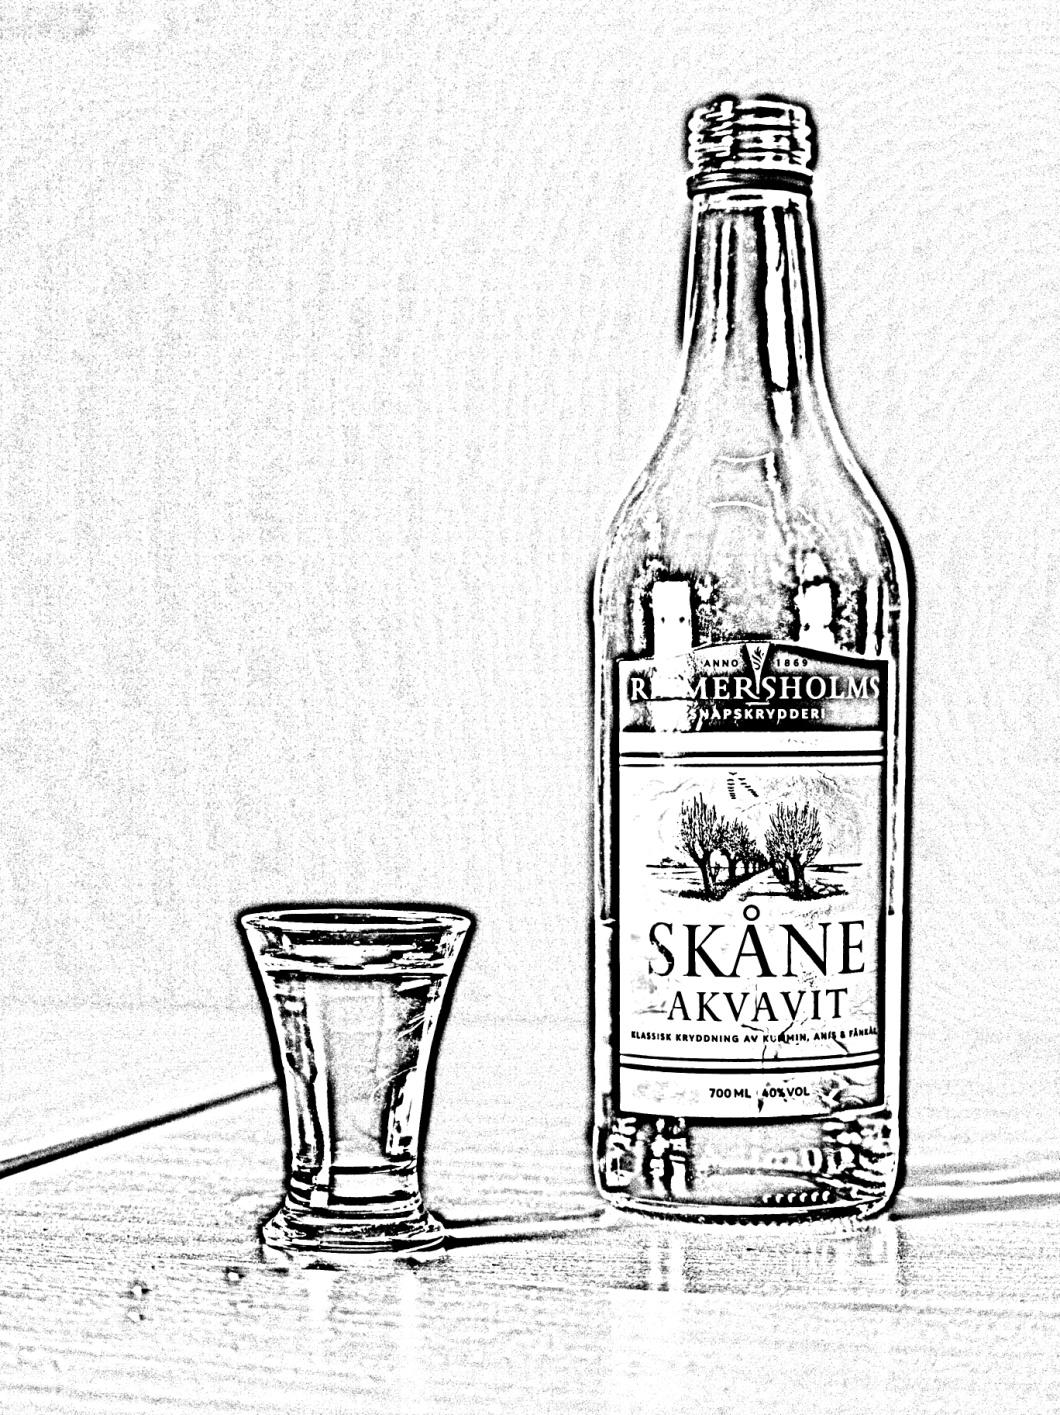
\includegraphics[width=0.8\textwidth]{res/snapsvisor.jpg}
   \section{Snapsvisor}
\end{center}
\vfill
\newpage

\subsection{1, 2, 75, 6, 7}
\textit{Mel: Ritsch, ratsch}\\
\index[alfa]{1, 2, 75, 6, 7}
\index[anfa]{1, 2, 75, 6, 7, 75...}
\begin{parse lines}[\noindent]{#1\\}

1, 2, 75, 6, 7, 75, 6, 7, 75, 6, 7,
1, 2, 75, 6, 7, 75, 6, 7, 73,
107, 103, 102, 107, 6, 19, 27,
17, 18, 16, 15, 13, 19, 14, 17,
19, 16, 18, 11, 8, 47.
\end{parse lines}

\subsection{Mera brännvin}
\textit{Mel: Internationalen}\\
\index[alfa]{Mera brännvin}
\index[anfa]{Mera brännvin i glasen...}
\begin{parse lines}[\noindent]{#1\\}

Mera brännvin i glasen,
mera glas på vårt bord,
mera bord på kalasen,
mer kalas på vår jord.

Mera jordar med måne,
mera månar i mars,
mera marscher till Skåne,
mera Skåne, Gud bevars, bevars, bevars!
\end{parse lines}

\newpage
\subsection{75:an}
\textit{Mel: 34:an}\\
\index[alfa]{75:an}
\index[anfa]{Våra tentor har vi flunkat...}
\begin{parse lines}[\noindent]{#1\\}

Våra tentor har vi flunkat
Vi har fått vår diagnos
Nu vår HB vi har dunkat
Vi ska hamna i hypnos
Det gör inget om det luktar
Som en flaska med klorin
För vi ska ju bara fukta
Våra läppar med vårt vin

Men sen är det slut på fina viner
Ja, nu ska vi korka upp vår sprit
Det ska halsas utav OP
Absolut och akvavit
Ja, jag tar farväl av hjärnans celler
Vaknar aldrig mer
Nu är det slut på fina viner
Nu ska sjuttifemman i magen ner!
\end{parse lines}

\newpage
\subsection{Änglahund}
\textit{Mel: Marseljäsen}\\
\textit{Sångarstriden 1991}\\
\index[alfa]{Änglahund}
\index[anfa]{Det står en hund på fjärde våningen...}
\begin{parse lines}[\noindent]{#1\\}

Det står en hund på fjärde våningen,
och den tänker hoppa ner.

BANZAÏ!

Det var en japanesisk självmordshund,
och den hoppar aldrig mer.
\end{parse lines}

\subsection{Armen i vinkel}
(Ramsa)\\
\index[alfa]{Armen i vinkel}
\index[anfa]{Armen i vinkel...}
\begin{parse lines}[\noindent]{#1\\}

Armen i vinkel,
blicken i skyn.
Så var det menat,
whisky och renat.
Vårt mål: alkohol,
skål för den som tål, SKÅL!
\end{parse lines}

\newpage
\subsection{Att fela är mänskligt}
\textit{Mel: Prästens lilla kråka}\\
\textit{Lundakarnevalen 2010}\\
\index[alfa]{Att fela är mänskligt}
\index[anfa]{Trampa på ett smådjur...}
\begin{parse lines}[\noindent]{#1\\}

Trampa på ett smådjur,
slakta gulligt rådjur,
måste göras rätt försiktigt...

Gifta sig med släkten,
stjäla ur kollekten,
det är FEL och det är viktigt!

$\vert\vert$: Men att sjunga en snutt,
och ta sig en hutt -
Det är bara RÄTT och riktigt! :$\vert\vert$
\end{parse lines}


\subsection{Dricka långsamt}
\textit{Mel: Här kommer Pippi Långstrump}\\
\index[alfa]{Dricka långsamt}
\index[anfa]{Visst kan man dricka långsamt...}
\begin{parse lines}[\noindent]{#1\\}

Visst kan man dricka långsamt,
hälla opp eller ner eller ingen ta.
Visst kan man dricka långsamt,
men det tänker inte jag!
\end{parse lines}


\subsection{Dansk snapsvisa}
\textit{Mel: Valfri}\\
\index[alfa]{Dansk snapsvisa}
\index[anfa]{Icke nu...}
\begin{parse lines}[\noindent]{#1\\}

Icke nu,
icke nu,
icke nu,
Men nu!
\end{parse lines}


\subsection{Finsk snapsvisa}
\textit{Mel: Ingen}\\
\index[alfa]{Finsk snapsvisa}
\index[anfa]{;)}
\begin{parse lines}[\noindent]{#1\\}

;)
\end{parse lines}

\newpage
\subsection{En gång i månan}
\textit{Mel: Mors lilla Olle}\\
\index[alfa]{En gång i månan}
\index[anfa]{En gång i månan är månen full...}
\begin{parse lines}[\noindent]{#1\\}

En gång i månan är månen full
Aldrig jag sett honom ramla omkull
Stum av beundran hur mycket han tål
Höjer jag glaset och utbringar en skål
\end{parse lines}


\subsection{Imsig vimsig}
\textit{Mel: Imse vimse spindel}\\
\index[alfa]{Imsig vimsig}
\index[anfa]{Imsig, vimsig blir man av en liten hutt...}
\begin{parse lines}[\noindent]{#1\\}

Imsig, vimsig blir man av en liten hutt.
Blodet börjar rusa, hjärtat tar en skutt.
Benen skälver, näsan den blir blå.
Fast det är så läskigt, vågar jag ändå!
\end{parse lines}


\subsection{Uddevalla}
\textit{Mel: Här går vägen till Uddevalla + Kärlek på lasarett}\\
\index[alfa]{Uddevalla}
\index[anfa]{Här går vägen till Uddevalla...}
\begin{parse lines}[\noindent]{#1\\}

Här går vägen till Uddevalla,
kärlek på lasarett.
Hej!
\end{parse lines}

\newpage
\subsection{Full idag}
\textit{Mel: My darling Clementine}\\
\index[alfa]{Full idag}
\index[anfa]{Full idag och full imorgon...}
\begin{parse lines}[\noindent]{#1\\}

Full idag och full imorgon,
så ser livet ut för mig.
Alla andra får varandra,
men jag ska aldrig gifta mig.

Rista in det på min gravsten.
Rista in det på latin.
Här vilar stoftet av en yngling,
som alltid varit ett fyllesvin
\end{parse lines}


\subsection{Lilla nubben}
\textit{Mel: Hej tomtegubbar}\\
\index[alfa]{Lilla nubben}
\index[anfa]{Tänk om jag hade lilla nubben...}
\begin{parse lines}[\noindent]{#1\\}

Tänk om jag hade lilla nubben
uppå ett snöre i halsen.
Tänk om jag hade lilla nubben
uppå ett snöre i halsen.
Jag skulle dra den upp och ner
så att det kändes som många fler.
Tänk om jag hade lilla nubben
uppå ett snöre i halsen.
\end{parse lines}

\subsection{Helangorakatt}
\textit{Mel: Vi gå över daggstänkta berg}\\
\index[alfa]{Helangorakatt}
\index[anfa]{Det var en gång en helangorakatt, fallera...}
\begin{parse lines}[\noindent]{#1\\}

Det var en gång en helangorakatt, fallera,
som älskade en vanlig bonnakatt, fallera.
Och följden blev en jamare,
fast den blev mycket tamare,
för den var bara halvangorakatt, fallera.
\end{parse lines}


\subsection{Vaktmästaren och professorn}
\textit{Mel: Internationalen}\\
\index[alfa]{Vaktmästaren och professorn}
\index[anfa]{Om vaktmästaren och professorn...}
\begin{parse lines}[\noindent]{#1\\}

Om vaktmästaren och professorn
de skulle byta lönegrad,
då blev professorn ganska ledsen,
men vaktmästaren blev glad.
\end{parse lines}
\vfill
\noindent\textit{Karnevalsfilmen 2002 baseras på denna visa och har ytterligare två strofer skrivna speciellt för filmen. De ursprungliga extra stroferna är förlorade i tiden.}



\newpage
\subsection{Helan går}
\textit{Mel: Helan går}\\
\index[alfa]{Helan går}
\index[anfa]{Helan går...}
\begin{parse lines}[\noindent]{#1\\}

Helan går,
sjung hopp faderallan lallan lej,
Helan går,
sjung hopp faderallan lej.
Och den som inte helan tar,
han heller inte halvan får.
Helan går,
sjung hopp faderallan lej.
\end{parse lines}

\noindent\textit{Visste du att svenskarna sjöng Helan går när vi vann VM i ishockey mot Sovjetunionen 1957 eftersom alla inte kunde nationalsången?}


\subsection{Hell and Gore}
\textit{Mel: Helan går}\\
\index[alfa]{Hell and Gore}
\index[anfa]{Hell and Gore...}
\begin{parse lines}[\noindent]{#1\\}

Hell and Gore
Chung Hop father Allan, Allan ley
Hell and Gore
Chung Hop father Allan ley

Oh handsome in the hell and tar
And hell are in the half and four
Hell and Gore...
Chung Hop father Allan ley
\end{parse lines}

\vspace{-0.9cm}
\subsection{Humlorna}
\textit{Mel: Karl-Alfred boy}\\
\index[alfa]{Humlorna}
\index[anfa]{Vi äro små humlor vi bzz, bzz...}
\begin{parse lines}[\noindent]{#1\\}

Vi äro små humlor vi bzz, bzz
Vi äro små humlor vi bzz, bzz
Vi äro små humlor som tar oss en geting
Vi äro små humlor vi bzz, bzz

Vi äro små fiskar vi blubb, blubb
Vi äro små fiskar vi blubb, blubb
Vi äro små fiskar som tar oss en kallsup
Vi äro små fiskar vi blubb, blubb

Vi äro små änglar vi flax, flax
Vi äro små änglar vi flax, flax
Vi äro små änglar som tar oss en Djävel
Vi äro små änglar vi flax, flax
\end{parse lines}

\vspace{-0.3cm}
\subsection{Utav brännvin}
\textit{Mel: Byssan lull}\\
\index[alfa]{Utav brännvin}
\index[anfa]{Byssan lull, utav brännvin blir han full...}
\vspace{-0.1cm}
\begin{parse lines}[\noindent]{#1\\}

Byssan lull, utav brännvin blir han full
och glammar och vill leva loppan.
Byssan lull, utav brännvin blir han full
och doppar sin slips uti soppan.
Han sliter och han drar
i stumpen som är kvar
men har ganska svårt att få opp'an!
\end{parse lines}

\vspace{-0.9cm}
\subsection{Nu är det fest igen}
\textit{Mel: Milord}\\
\index[alfa]{Nu är det fest igen}
\index[anfa]{Nu är det fest igen...}
\begin{parse lines}[\noindent]{#1\\}

Nu är det fest igen
i vårat glada gäng
och vi behöver inte ta några poäng.
För CSN är skit
vi tillhör den elit
som låter farsan pröjsa för all våran sprit!
\end{parse lines}


\subsection{Nubben}
\textit{Mel: Camptown races}\\
\index[alfa]{Nubben}
\index[anfa]{Alla vet; i glaset finns...}
\begin{parse lines}[\noindent]{#1\\}

Alla vet; i glaset finns
nubben, nubben.
Den som inte nubben minns,
han har skoj ändå.
Nubben känns igen som en gammal vän.
In i gapet åker den, käften slår igen.
\end{parse lines}
\textit{(klapp)}

\newpage
\subsection{Nu dags taga sig en snaps strax}
\textit{Mel: Can-can}\\
\index[alfa]{Nu dags taga sig en snaps strax}
\index[anfa]{Nu dags taga sig en snaps strax...}
\begin{parse lines}[\noindent]{#1\\}

Nu dags taga sig en snaps strax,
som din kropp tar opp och låter rinna ner.
Och ger dig smak för flera

Ditt liv, blott ett tidsfördriv,
du kastar ner en kask och lever glatt och ler,
när fler du ser.

Med sill, eller vad du vill till,
håll din strupe våt, åt Bacchus ge din själ,
han vill dig bara väl.

Så skjut först en kort salut ut
nu tar sången slut, trut.
Gapa, svälj och njut!
\end{parse lines}

\newpage
